% Escala logarítmica: x = 2,6 log10(masa en g), origen en 1 g.
% Filas separadas 0,75 cm. Un punto indica una sola masa por dosis.
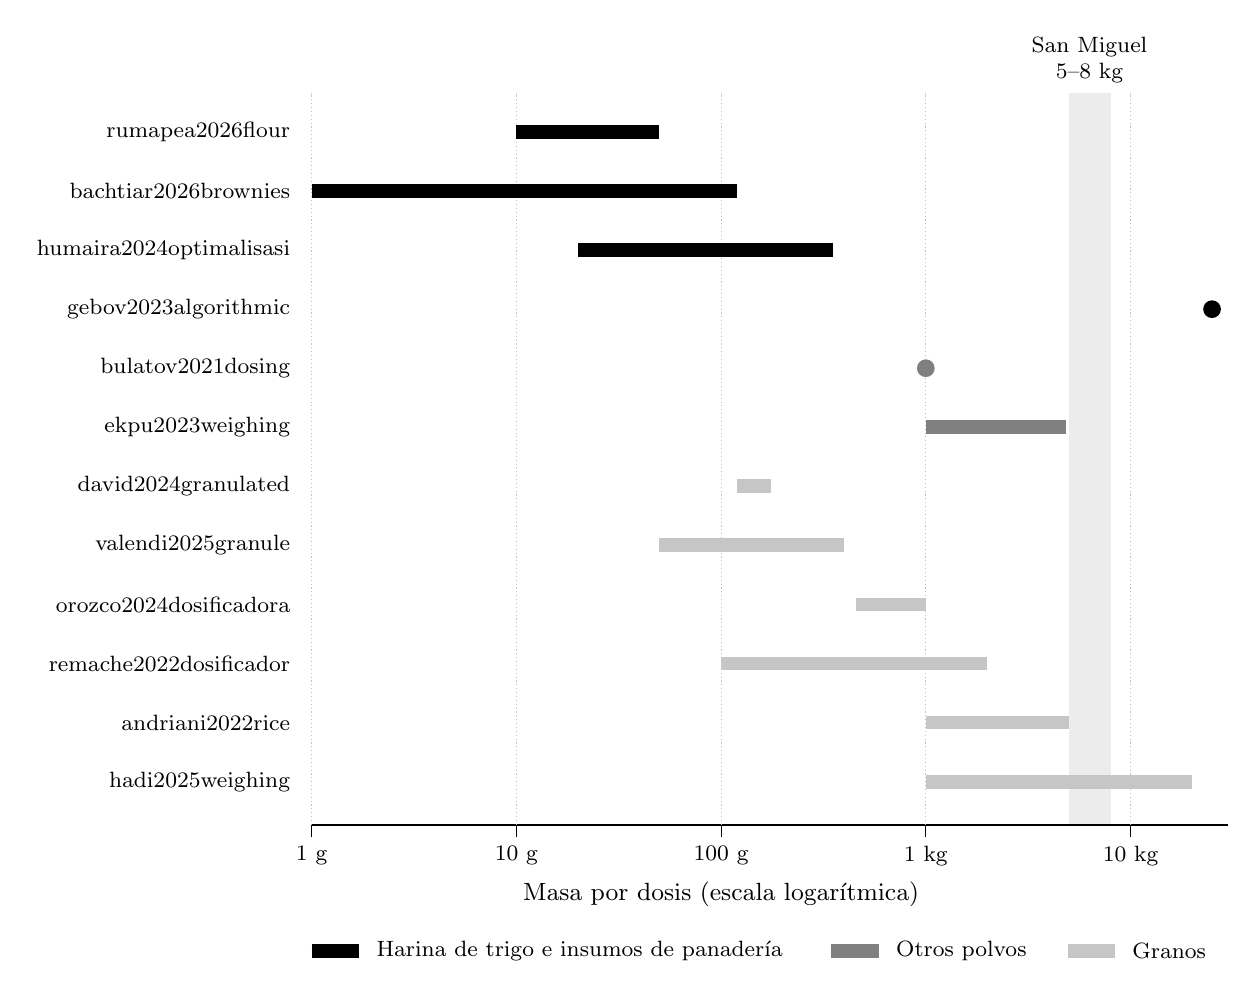
\begin{tikzpicture}[font=\small, nota/.style={font=\footnotesize}]
% Banda de la Panadería San Miguel: 5 a 8 kg
\fill[gray!15] (9.617,0.2) rectangle (10.148,9.5);
\node[nota, align=center, anchor=south] at (9.878,9.5) {San Miguel\\5--8~kg};
% Eje
\draw[thick] (0,0.2) -- (11.641,0.2);
\draw (0.0,0.2) -- (0.0,0.05);
\node[nota, below] at (0.0,0.05) {1~g};
\draw[gray!50, densely dotted] (0.0,0.2) -- (0.0,9.5);
\draw (2.6,0.2) -- (2.6,0.05);
\node[nota, below] at (2.6,0.05) {10~g};
\draw[gray!50, densely dotted] (2.6,0.2) -- (2.6,9.5);
\draw (5.2,0.2) -- (5.2,0.05);
\node[nota, below] at (5.2,0.05) {100~g};
\draw[gray!50, densely dotted] (5.2,0.2) -- (5.2,9.5);
\draw (7.8,0.2) -- (7.8,0.05);
\node[nota, below] at (7.8,0.05) {1~kg};
\draw[gray!50, densely dotted] (7.8,0.2) -- (7.8,9.5);
\draw (10.4,0.2) -- (10.4,0.05);
\node[nota, below] at (10.4,0.05) {10~kg};
\draw[gray!50, densely dotted] (10.4,0.2) -- (10.4,9.5);
\node[anchor=north] at (5.2,-0.4) {Masa por dosis (escala logarítmica)};
% Filas: intervalo de masa por dosis de cada fuente
\draw[line width=5pt, black] (2.6,9.0) -- (4.417,9.0);
\node[nota, anchor=east] at (-0.15,9.0) {\textcite{rumapea2026flour}};
\draw[line width=5pt, black] (0.0,8.25) -- (5.406,8.25);
\node[nota, anchor=east] at (-0.15,8.25) {\textcite{bachtiar2026brownies}};
\draw[line width=5pt, black] (3.383,7.5) -- (6.615,7.5);
\node[nota, anchor=east] at (-0.15,7.5) {\textcite{humaira2024optimalisasi}};
\fill[black] (11.435,6.75) circle (3.2pt);
\node[nota, anchor=east] at (-0.15,6.75) {\textcite{gebov2023algorithmic}};
\fill[gray] (7.8,6.0) circle (3.2pt);
\node[nota, anchor=east] at (-0.15,6.0) {\textcite{bulatov2021dosing}};
\draw[line width=5pt, gray] (7.8,5.25) -- (9.576,5.25);
\node[nota, anchor=east] at (-0.15,5.25) {\textcite{ekpu2023weighing}};
\draw[line width=5pt, gray!45] (5.406,4.5) -- (5.832,4.5);
\node[nota, anchor=east] at (-0.15,4.5) {\textcite{david2024granulated}};
\draw[line width=5pt, gray!45] (4.417,3.75) -- (6.765,3.75);
\node[nota, anchor=east] at (-0.15,3.75) {\textcite{valendi2025granule}};
\draw[line width=5pt, gray!45] (6.908,3.0) -- (7.8,3.0);
\node[nota, anchor=east] at (-0.15,3.0) {\textcite{orozco2024dosificadora}};
\draw[line width=5pt, gray!45] (5.2,2.25) -- (8.583,2.25);
\node[nota, anchor=east] at (-0.15,2.25) {\textcite{remache2022dosificador}};
\draw[line width=5pt, gray!45] (7.8,1.5) -- (9.617,1.5);
\node[nota, anchor=east] at (-0.15,1.5) {\textcite{andriani2022rice}};
\draw[line width=5pt, gray!45] (7.8,0.75) -- (11.183,0.75);
\node[nota, anchor=east] at (-0.15,0.75) {\textcite{hadi2025weighing}};
% Leyenda
\begin{scope}[shift={(0,-1.4)}]
    \draw[line width=5pt, black] (0,0) -- (0.6,0); \node[nota, anchor=west] at (0.7,0) {Harina de trigo e insumos de panadería};
    \draw[line width=5pt, gray] (6.6,0) -- (7.2,0); \node[nota, anchor=west] at (7.3,0) {Otros polvos};
    \draw[line width=5pt, gray!45] (9.6,0) -- (10.2,0); \node[nota, anchor=west] at (10.3,0) {Granos};
\end{scope}
\end{tikzpicture}
